%AOSD Modularity Visions Paper
\documentclass{acm_proc_article-sp}
\usepackage{color}
\usepackage{graphicx}
\usepackage{listings, tikz, xcolor}
\usepackage{bold-extra}
\usepackage{subfig}
\usepackage{enumerate}
\usepackage{courier}
\usepackage{syntax}
\usepackage{amsmath}
\usepackage{hyperref}
\usepackage{MnSymbol}
\lstset{ 
	language = [AspectJ]Java,
  basicstyle=\sffamily\small,
  numbers=left,
	numberstyle=\tiny\color[rgb]{0.25,0.25,0.25},
	numberblanklines=false,
  firstnumber=auto,
	breaklines=true,
  tabsize=2,
	emph={aspect,declare, adapter, instance, pointcut, adaptee, adapts, select, UNTIL,pc, instanceType, exp, removeExp}, 
	emphstyle=\textbf,
	escapechar={~},
	showstringspaces= false,
	frame=single,
	captionpos = b,
	numberbychapter=false,
	breakatwhitespace = true,
	columns=fullflexible
	}
\lstset{prebreak=\raisebox{0ex}[0ex][0ex]{\ensuremath{\rhookswarrow}}} % requires \usepackage{MnSymbol}
%\lstset{postbreak=\raisebox{0ex}[0ex][0ex]{\ensuremath{\rcurvearrowse\space}}} % requires \usepackage{MnSymbol}	
	
\usetikzlibrary{arrows,shapes.multipart,shapes.arrows,shapes.misc,calc,fit,shadows,positioning,patterns} 

\newcommand\bh{\tikz[remember picture]
					\node (begin highlight) {};
			 }
  \newcommand\eh{\tikz[remember picture]
		 \node (end highlight) {};
		 \tikz[remember picture, overlay] 
		 \draw[yellow,line width=10pt,opacity=0.3] (begin highlight) -- (end
			highlight);
		 }

\newcommand{\lstinlineabstract}[1]{\lstinline[emph={#1},emphstyle=\textit]{#1}}

\begin{document}

\title{Adapter Paper}

\numberofauthors{1}
\author{
\alignauthor
Kardelen Hatun \hspace{2cm} Christoph Bockisch \hspace{2cm} Mehmet Ak\c{s}it\\
\affaddr{TRESE, University of Twente, 7500AE Enschede, The Netherlands}\\
\affaddr{\url{http://www.utwente.nl/ewi/trese/}}\\
\email{ \{hatunk,c.m.bockisch,aksit\}@ewi.utwente.nl}
}
\maketitle

\begin{abstract}
This paper provides a sample of a \LaTeX\ document which conforms to
the formatting guidelines for ACM SIG Proceedings.
It complements the document \textit{Author's Guide to Preparing
ACM SIG Proceedings Using \LaTeX$2_\epsilon$\ and Bib\TeX}. This
source file has been written with the intention of being
compiled under \LaTeX$2_\epsilon$\ and BibTeX.

The developers have tried to include every imaginable sort
of ``bells and whistles", such as a subtitle, footnotes on
title, subtitle and authors, as well as in the text, and
every optional component (e.g. Acknowledgments, Additional
Authors, Appendices), not to mention examples of
equations, theorems, tables and figures.

To make best use of this sample document, run it through \LaTeX\
and BibTeX, and compare this source code with the printed
output produced by the dvi file.
\end{abstract}

% A category with the (minimum) three required fields
\category{H.4}{Information Systems Applications}{Miscellaneous}
%A category including the fourth, optional field follows...
\category{D.2.8}{Software Engineering}{Metrics}[complexity measures, performance measures]

\terms{Theory}

\keywords{ACM proceedings, \LaTeX, text tagging} % NOT required for Proceedings


\section{Introduction / Copied from SLE DocSym paper}
Complex systems are created by assembling software components of various types
and functions. Reuse is essential and
components created for a system are required to continue working after the system has
evolved. Some components may be
domain-specific, meaning their structure and functionality can be defined using
the fundamental concepts of the relevant domains. A domain-specific language
(DSL) provides expressive power over a particular domain. It allows software
development with high-level specifications; if general-purpose programming languages
are used, development may take a considerable programming effort. 

The specifications written in a DSL can be processed in various ways. These are
comprehensively described in \cite{Mernik:whenandhow} and
\cite{fowler2010domain}. Generative programming \cite{Czarnecki:overview} is one
of the processing options and has become highly popular with the emergence of
user-friendly language workbenches. Most language workbenches provide a means
to develop a compiler for the DSL, facilitating code generation in general-purpose
languages. (A comparison matrix for language workbenches can be found in
\cite{LWC}.) 

In this paper we focus on the integration of components into target systems.
``Component'' is a very general concept and it can be realized in different forms,
depending on the system. We particularly focus on a subset of components,
\emph{domain-specific components}, which are instances of domain-specific meta-models.
The component structure is described with a DSL and the semantics are embedded
into code generation templates, which are used to generate a component according to a predefined software architecture.
  

Integrating a generated component into a system poses three main chall enges.
(1) When adding unforeseen functionality to a
system, no explicit hooks exist for attaching the
generated component. In this case it may be necessary to modify the
generated code, the system code or both to make the connection, which will
expose the developer to the generated code, defying the purpose of code
generation. 
(2) The interfaces of the generated component and the target system should be compatible to work together, which is generally not the case. Then one of the interfaces should be adapted, possibly by modifying the system's or the component's implementation or their type-system.
(3) When the component or the target system evolves, the links between them
must be re-established. 



Current aspect-oriented languages offer mechanisms to modularly implement solutions for the first challenge. It can be solved by defining pointcuts that are used as hooks to a system. The second challenge is our main focus. Existing AO-languages offer limited mechanisms for implementing adapters between interfaces. AspectJ inter-type declarations can be used to make system classes to implement appropriate interfaces, however this approach is type-invasive. CaesarJ offers a more declarative approach with \emph{wrappers}, but their instantiation requires pointcut declarations or they should be explicitly instantiated in the base system. The links mentioned in the third challenge  are the adapter implementations mentioned in the second challenge and they represent the binding between two components. However current AO languages do not offer a declarative way for describing such a binding; an imperative programming language will lead to less readable and less maintainable implementation, which is fragile against software evolution.

\section{Approach}
In order to overcome the shortcomings of the existing approaches we intend to design a declarative way of implementing object adapters which is used together with a specialized pointcut for selecting objects. The object adapter pattern is common practice for binding two components that have incompatible interfaces. Our approach is aspect-oriented and it will provide the means to non-intrusively define and instantiate object adapters, inside aspects. These adapters represent links between the component and the system; their declarative design requires a declarative way of selecting the adaptee objects. 

\subsection{Adaptee Selection}
The object adapter pattern relies on either getting the adaptee object as a parameter at construction or setting the adaptee object after construction. This approach requires acquiring adaptee objects and explicitly initializing the object adapters. 
Unlike inter-type declarations, adapter declarations are not type invasive; they do not change the type hierarchy of the contained object. They also do not require explicit instantiations. 
There are two ways to pass on the adaptee objects to an adapter declaration. First is referencing a collection instance which contains a set of objects to be adapted. This method is straightforward but limited in terms of object selection options.
The second method uses a new pointcut mechanism that we have designed called \emph{instance pointcut} which selects sets of objects based on the execution history.
An instance pointcut definition consists of three parts: an identifier, a type which is the upper bound for all objects in the selected set, and a specification of relevant objects.
The specification utilizes \emph{pointcut expressions} to select events that define the begin and end of life-cycle phases and to expose the object.
At these events, an object is added or removed from the set representing the instance pointcut.
It is possible to access all objects currently selected by an instance pointcut and to
be notified, when an object is added or removed.

New instance pointcuts can be derived from existing ones in several ways. Firstly, a new instance pointcut can be derived from another one by restricting the type of selected objects. Secondly, instance pointcut declarations can be composed arbitrarily by means of boolean operators. Adapter declarations refer to the sets selected by instance pointcuts, and automatically instantiate adapters for each object in the referred set.


\subsection{Adapter Declarations}
\label{adintro}

Adapter declarations are contained by aspects but like inter-type declarations they are not aspect members. In Figure~\ref{basicgram} the basic syntax of adapter declarations are shown. 
The header of an adapter declaration consists of an identifier (Figure~\ref{basicgram}: $\langle identifier \rangle$), the list of interfaces the adapter implements (Figure~\ref{basicgram}: $\langle interface \rangle+$) and an adaptee reference which contains the adaptee objects. In the body of an adapter declaration implementation of the interface methods is provided. In the body of an adapter declaration, the keyword \textsf{adaptee} corresponds to the object that's being adapted. 

\begin{figure}[h!]
\begin{grammar}
<concrete-adapter-decl> ::= `declare adapter:' <identifier> `[' <interface>+ `]' `adapts' <adaptee-ref> `{'
<adapter-body> `}'

<adaptee-ref> ::= <ip-ref> \alt <obj-collection>
\end{grammar}
\caption{Grammar definition for adapter declarations}
\label{basicgram}
\end{figure}

Let us give a concrete example to illustrate how adapter declarations can be used. In Figure~\ref{fig:shapes} a \textsf{Shape} hierarchy and the interfaces offered by the classes in this hierarchy is shown. The \textsf{ShapeInfo} class uses \textsf{ShapeArea} and \textsf{ShapeCircumference} interfaces to query existing \textsf{Shape}s (Figure~\ref{fig:shapeint}). However none of the classes in the shapes hierarchy implements these interfaces, hence they should be adapted. 


\begin{figure}[ht]
\subfloat[The shapes hierarchy]{
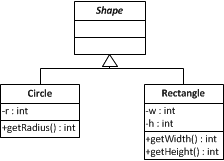
\includegraphics[width=0.44\columnwidth]{images/shapes.png}
\label{fig:shapes}
}
\hspace{10pt}
\subfloat[ShapeInfo class that requires two unsupported interfaces]{
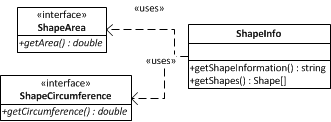
\includegraphics[width=0.44\columnwidth]{images/shapeint.png}
\label{fig:shapeint}
}
\caption{Incompatible interfaces: Shape and ShapeInfo}
\label{fig:shapeinfo}
\end{figure}

Assume that we have defined an instance pointcut called \textsf{circles} which selects the set of \textsf{Circle} objects that are created. Listing~\ref{circleadapter} shows an example of an adapter declaration named \textsf{CircleAdapter} and which implements \textsf{ShapeArea} and \textsf{ShapeCircumference} interfaces (Line~\ref{caheader}). \textsf{CircleAdapter} adapts the objects selected by the \textsf{circles} instance pointcut. In the body of the adapter the method implementations are shown. The first method \textsf{getArea} returns the area of the \textsf{adaptee} which is of type \textsf{Circle}, by calling \textsf{adaptee}'s \textsf{getRadius} method (Lines~\ref{ca:area:begin}~--~\ref{ca:area:end}). The \textsf{getCircuference} method from \textsf{ShapeCircumference} interface is similarly implemented (Lines~\ref{ca:circ:begin}~--~\ref{ca:circ:end}).



\begin{lstlisting}[float, label={circleadapter}, caption={The adapter declaration for \textsf{Circle} objects}]
declare adapter: CircleAdapter[ShapeArea, ShapeCircumference] adapts circles ~\label{caheader}~
{
	public double getArea()~\label{ca:area:begin}~
	{
		return Math.pow(adaptee.getRadius(),2)*Math.PI;
	}~\label{ca:area:end}~
	public double getCircumference()~\label{ca:circ:begin}~
	{
		return 2*adaptee.getRadius()*Math.PI;
	}~\label{ca:circ:end}~
}
\end{lstlisting} 



\subsubsection{Adapter Hierarchies}

Similar to Java classes, adapter declarations can also form inheritance hierarchies. The extended grammar that support adapter inheritance is given in Figure~\ref{adaphier}. According to this grammar extension three types of adapter declarations are possible. 

\begin{figure}[h!]
\begin{grammar}
<adapter-decl> ::= <abstract-adapter-decl> \alt <concrete-adapter-decl> \alt <adapter-extend-decl>

<abstract-adapter-decl> ::= `declare adapter:' 'abstract' <identifier> `[' <interface>+ `]'  (`adapts' <adaptee-ref> | <type-ref>)? `{' <adapter-body>? `}'

<adapter-extend-decl> ::= `declare adapter:' <identifier>(`[' <interface>+ `]')? `extends' <adapter-ref> `adapts' <adaptee-ref> `{' <adapter-body> `}'

\end{grammar}
\caption{Extended grammar definition for adapter hierarchies}
\label{adaphier}
\end{figure}

\begin{description}
	\item[Abstract Adapter Declaration] An abstract adapter declaration ($\langle \text{abstract-adapter-decl}\rangle$ rule) takes the \textsf{abstract} keyword before its identifier. Such declarations do not have to provide an advice body or they can provide a partial adapter body, which implements only some methods of the declared interfaces. Different form concrete adapter declarations, the adaptee does not have to be bound. Adaptee reference can either be empty, or an adapter reference ($\langle \text{adaptee-ref}\rangle$ rule in Figure~\ref{basicgram}) or it can be a \emph{type reference}, in order to constrain the bound type for the concrete sub-adapter.
	\item[Extended Adapter Declaration] An adapter can extend other adapters, either abstract or concrete. An extended adapter can override the interface methods defined by its super-adapter and implement new interfaces. However there are some rules when extending adapters. 
	\begin{itemize}
		\item Extending an abstract adapter requires that all of the interface methods that are not implemented in the super-abstract adapter should be implemented by the sub-adapter, given that the sub-adapter is concrete. 
		\item If the abstract super-adapter uses a type-reference in place of the adaptee, then the sub-adapters can only bind adaptees that are subtypes of the declared type-reference.
		\item If the super-adapter uses an instance pointcut reference as the adaptee, then the sub-adapters can only bind the type-refined subsets of that instance pointcut. \textbf{Alternative: the sub-adapters can only bind the subtypes of the instance pointcut's declared type.} This rule also hold for the plain object collections.
	\end{itemize}
	The typing constraints still hold if the sub-adapter is abstract, however the first rule does not apply.
	\item[Concrete Adapter Declaration] Concrete adapter declaration was discussed in subsection \ref{adintro}.
\end{description}
 
Using the shapes example presented in Figure~\ref{fig:shapeinfo}, we can illustrate how adapter hierarchies can be utilized. In Listing~\ref{lst:absshapes}, line~\ref{caheader2} an abstract adapter which adapts \textsf{Shape} objects is shown, here the instance pointcut \textsf{shapes} selects all created \textsf{Shape} objects.
The \texttt{ShapeAdapter} contains an implementation of the \texttt{ShapeColor} interface, which will be a common implementation for all the sub-adapters if not overridden. 
The \texttt{getColor} method (lines~\ref{gc:begin}~--~\ref{gc:end}) calls the \texttt{getArea} method (line~\ref{gc:if}) of the \texttt{ShapeArea} interface. When this method is called on the concrete sub-adapters, each sub-adapter will call its own \texttt{getArea} implementation. 
On line~\ref{sh:circle:begin} we have defined a \textsf{CircleAdapter} which extends the abstract \textsf{ShapeAdapter}. \textsf{CircleAdapter} does not have to declare an interface list since it is a sub-adapter and it inherits the interfaces from its super-adapter. 
Another important point is the way we refined the \textsf{shapes} instance pointcut with a Java generics type syntax. 
By writing \textsf{shapes<Circle>} we can select the \textsf{Circle} instances from the instance pointcut set and bind the specialized \textsf{CircleAdapter} to these objects.

\begin{lstlisting}[float, label={lst:absshapes}, caption={An abstract adapter declaration for the \textsf{Shape} hierarchy}]
declare adapter: abstract ShapeAdapter[ShapeArea, ShapeCircumference, ShapeColor] adapts shapes ~\label{caheader2}~
{
	public String getColor(){~\label{gc:begin}~
			if (this.getArea() > 40) ~\label{gc:if}~
				return "RED";
			else
				return "BLUE";
		}~\label{gc:end}~
}
declare adapter: CircleAdapter extends ShapeAdapter adapts shapes<Circle> { ~\label{sh:circle:begin}~
	//implementation of interface methods for a circle
} ~\label{sh:circle:end}~

declare adapter: RectangleAdapter extends ShapeAdapter  adapts shapes<Rectangle>{~\label{sh:rect:begin}~
	//implementation of interface methods for a rectangle
}~\label{sh:rect:end}~
\end{lstlisting} 

\subsection{Adapter Compilation}
Adapter declarations are compiled to Java classes and Aspects. \textbf{Some meta-information is attached to the generated code in order to be used during run-time(?).} The transformation of an adapter declaration to a Java class is straight-forward. For the example given in Listing~\ref{lst:absshapes} the Java classes shown in Listing~\ref{lst:absshapesjava} are generated. 

\begin{lstlisting}[float, label={lst:absshapesjava}, caption={The generated Java code from the adapter declarations in Listing~\ref{lst:absshapes}}]
public abstact class ShapeAdapter implements ShapeArea, ShapeCircumference, ShapeColor { 
{
	Shape adaptee;
	ShapeAdapter(Shape s)
	{
		adaptee = s;
	}
	public String getColor(){
		if (this.area() > 40)
			return "RED";
		else
			return "BLUE";
	}	
}
public class CircleAdapter extends ShapeAdapter{
	Circle adaptee;
	public CircleAdapter(Circle c)
	{
		super(c);
		adaptee = c;
	}
	//implementation of interface methods for a circle
}
public class RectangleAdapter extends ShapeAdapter{
	Rectangle adaptee;
	public RectangleAdapter(Rectangle r)
	{
		super(r);
		adaptee = r;
	}
	//implementation of interface methods for a rectangle
}
\end{lstlisting} 


%
%\section{Compilation and Run-time Support}
%In our prototype implementation instance pointcuts are compiled to AspectJ code. Roughly, an instance pointcut is transformed to several AspectJ pointcuts, advice declarations and a set structure.  Adapter declarations will also be compiled to AspectJ. According to our initial analysis an adapter declaration will map to a Java class for the adapter and advice bodies for initializing adapters. These advice bodies will reference the pointcuts generated from the instance pointcut which is referenced by the adapter declaration. 
%
%We intend to provide run-time support for retrieving adapter instances. Adapters are automatically initialized when an adaptee object satisfying the referenced instance pointcut's conditions become available. These adapter instances can be indexed and accessed through a run-time library. To do this, we have the requirement that the results of a retrieval will always be non-ambiguous e.g. if a query to retrieve a single adapter instance, matches two adapters, then there should be appropriate resolution mechanisms or user feedback to overcome the issue. 









\bibliographystyle{splncs}
\bibliography{main}




\end{document}